\section{Final Platform Design}
\begin{figure}[H]
    \centering
    \includegraphics[page = 2,width=0.59\textwidth]{design/platform_showcase/platform_drawings.pdf}
    \caption{Complete assembly of a platform in Onshape. \href{https://cad.onshape.com/documents/0d531e009de73b9ed4692d36/w/83d10e6192a92a79ef75f390/e/35ebef400ac87f1073d7eabc?renderMode=0&uiState=6a06f9cc76a0e4c598c450d3}{Project link}}
\end{figure}
For the testing purposes, the platform with the tilt angle of \SI{64}{\degree} was designed.
The exploded view shown in \cref{fig:exploded_view} illustrates all the components of the platform and their arrangement. 

The hole located on the underside of the platform mount is intended for the insertion of a magnet used for the platform homing procedure.
Two rectangular extensions positioned on opposite sides of the ring gear are used for mounting the microcontroller and the Hall effect sensor.
Two holes are present in the base of the ring gear. The central hole is meant for the insertion of the stepper motor shaft, while the hole located near one of the rectangular extensions is used for routing wires supplying power to the microcontroller and the \gls{lidar} sensor, as well as wires used for controlling the stepper motor driver.
\begin{figure}
    \centering
    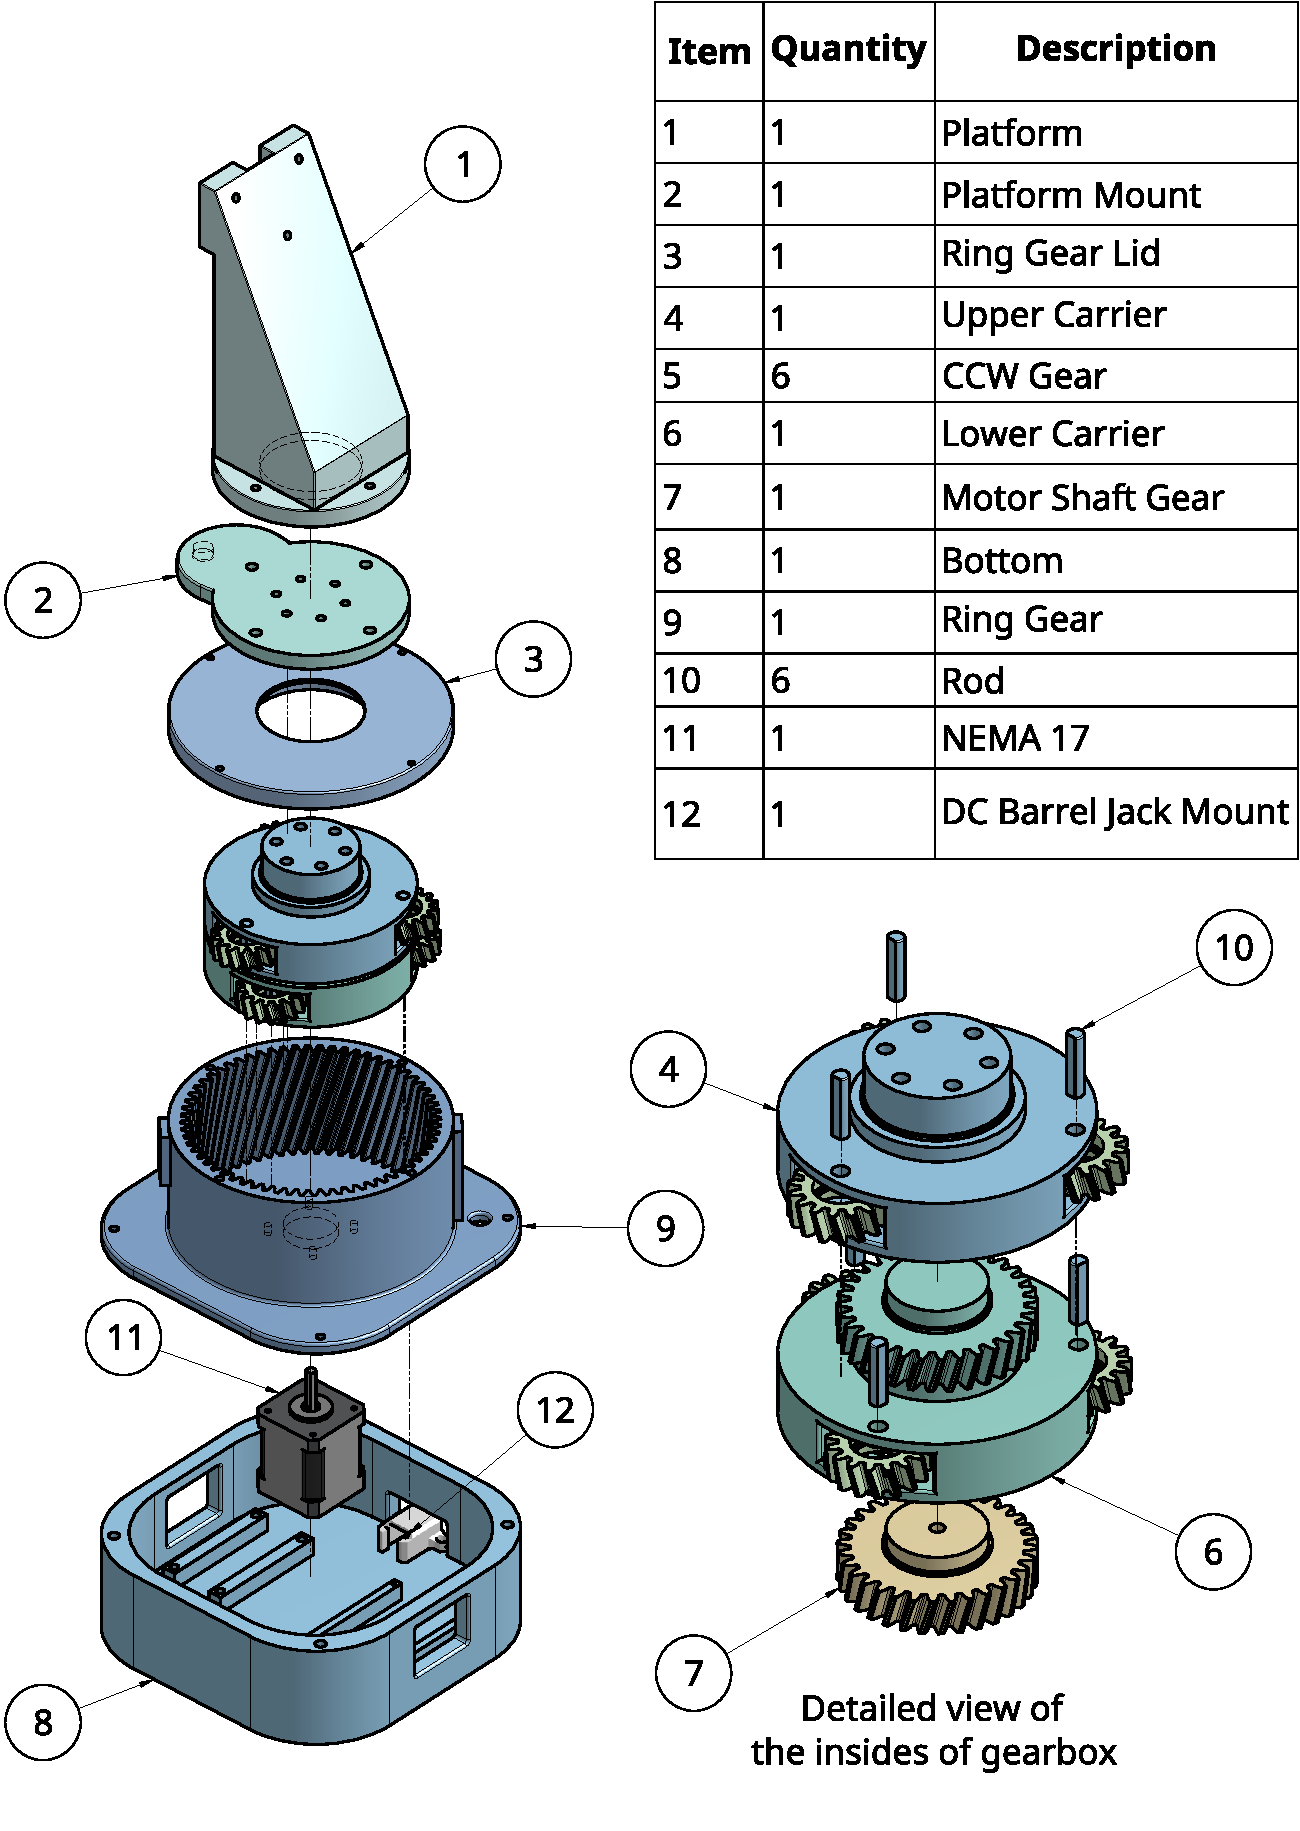
\includegraphics[page = 1,width=\textwidth]{design/platform_showcase/platform_drawings.pdf}
    \caption{Exploded view of the platform}
    \label{fig:exploded_view}
\end{figure}
\begin{figure}
    \centering
    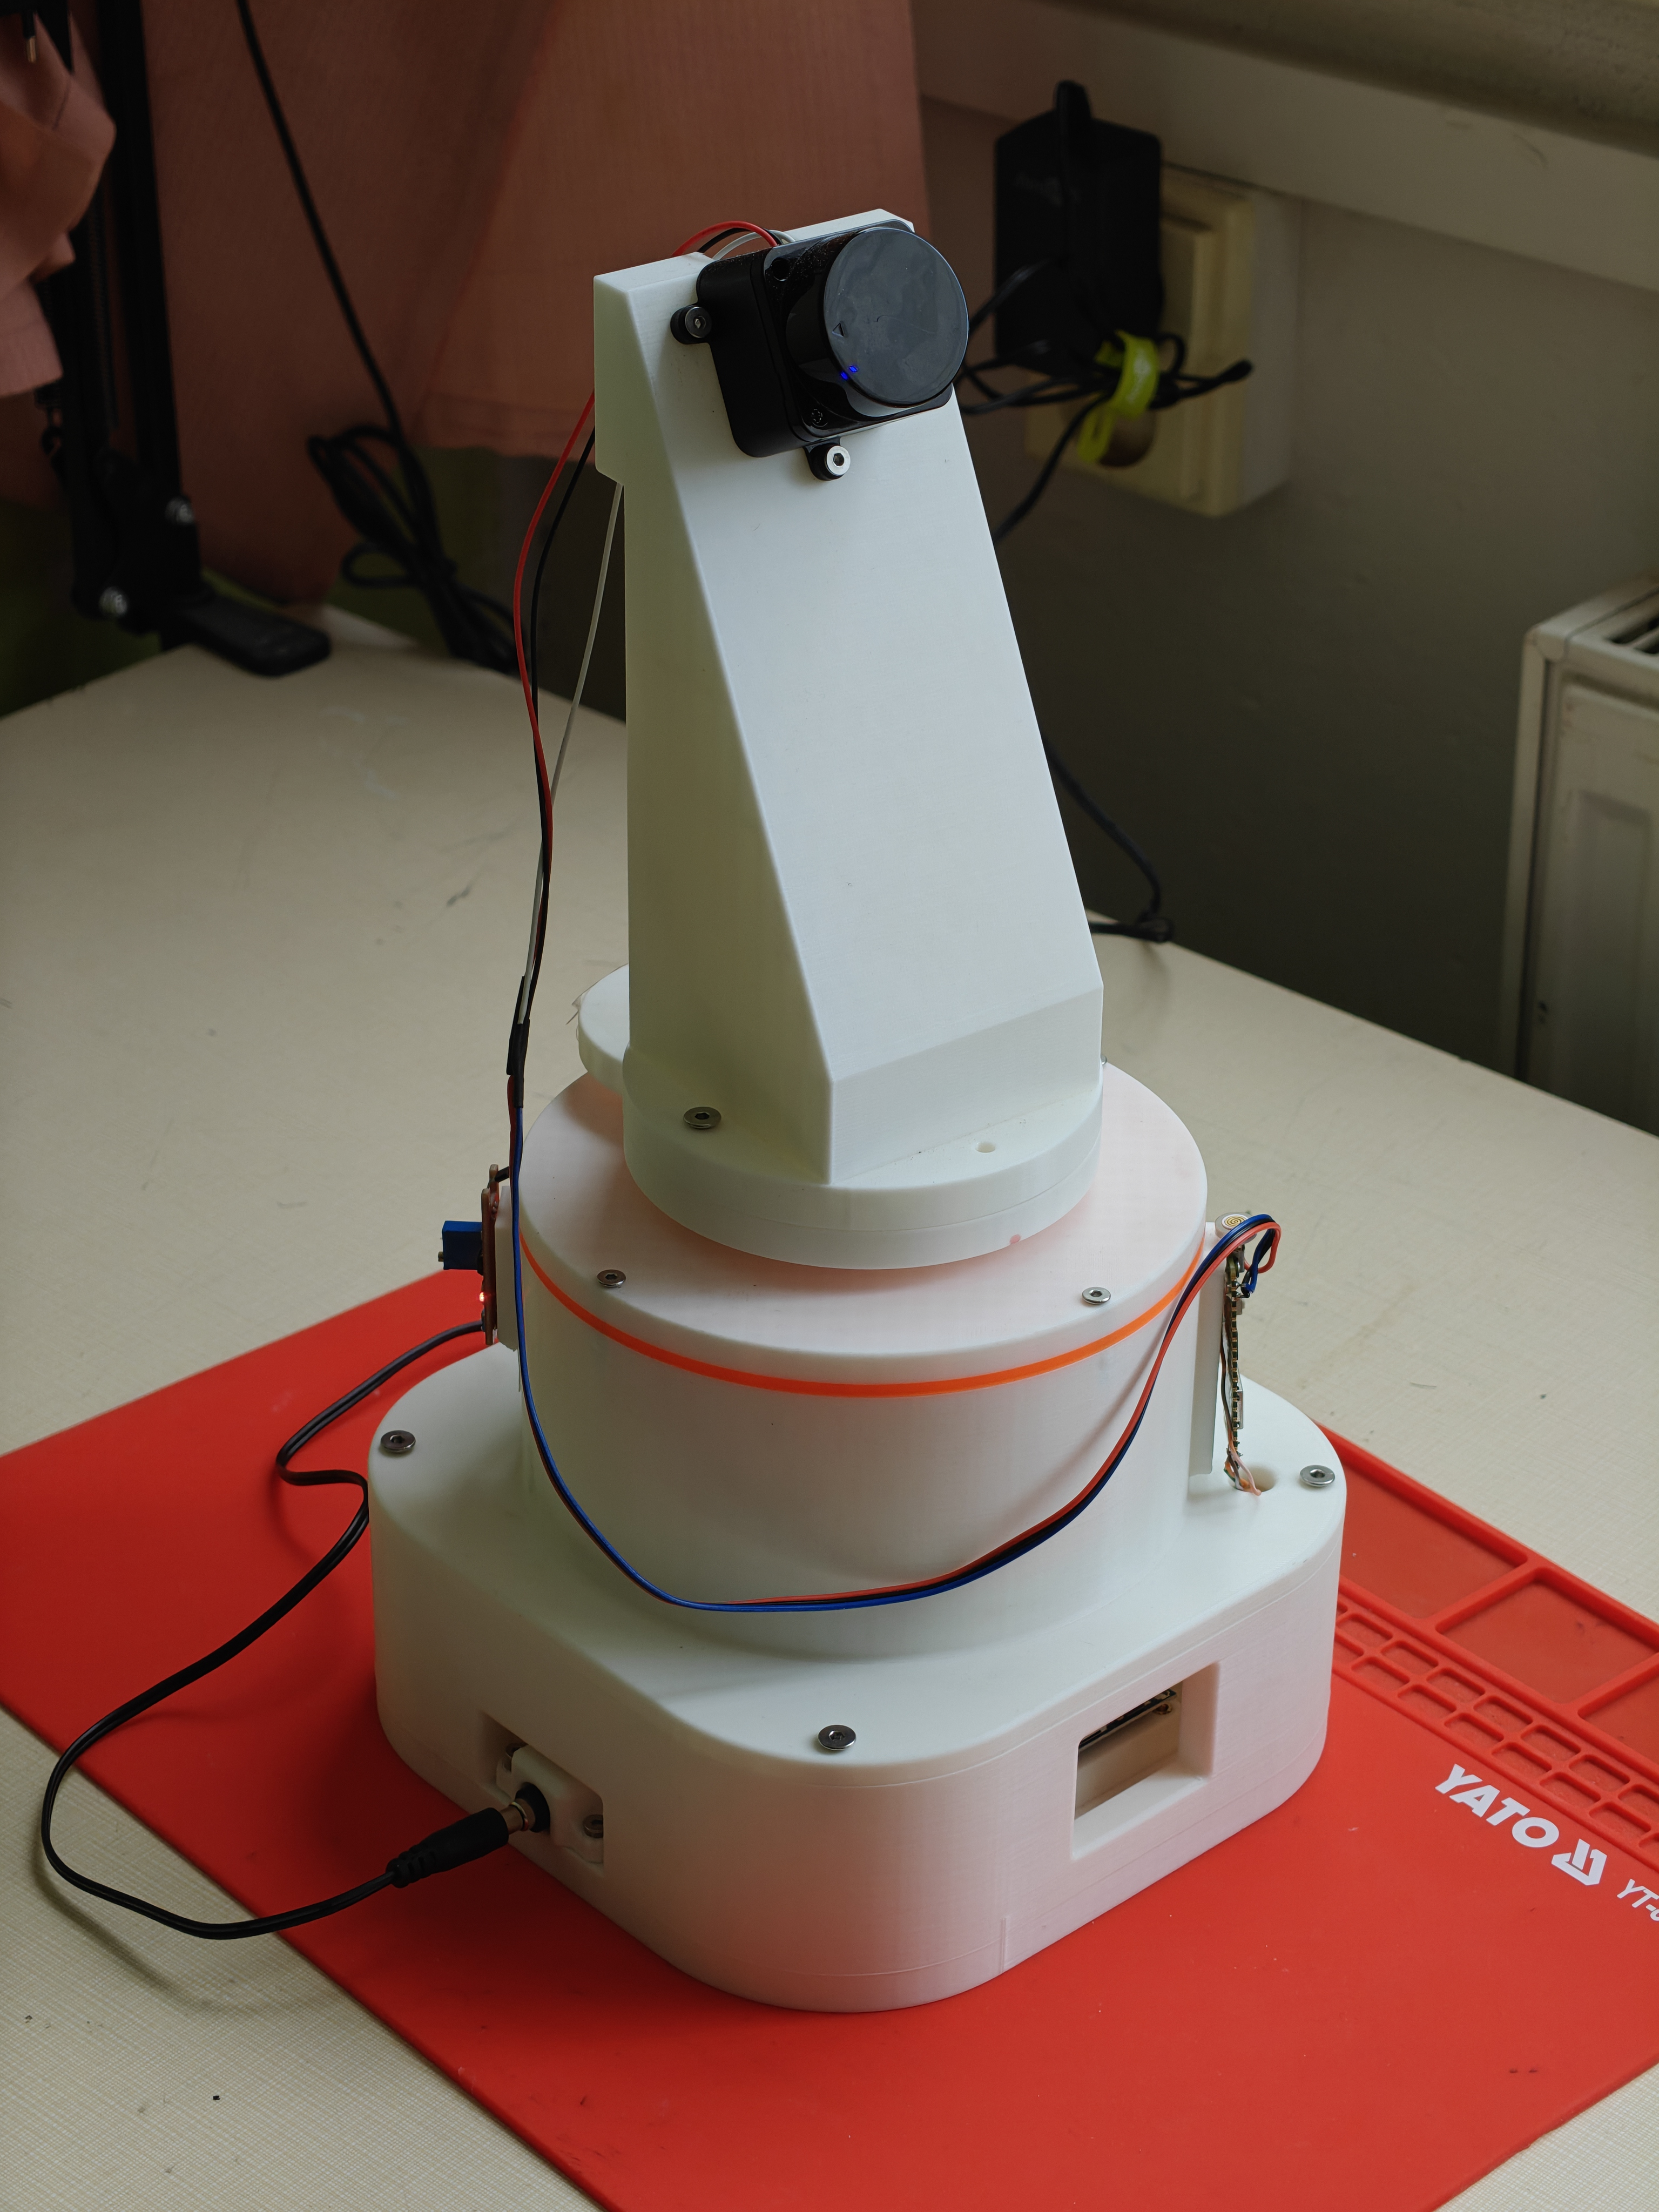
\includegraphics[width=\textwidth]{design/platform_showcase/platform_photo.jpg}
    \caption{Photo of the assembled platform}
\end{figure}